\chapter{Equações}
%\label{cap:0}

\colorbox{azul}{
 \begin{minipage}{0.9\linewidth}
 \begin{center}
   Uma equação é uma sentença matemática aberta, ou seja, sentença matemática que possui ao menos uma incógnita, e que estabelece uma igualdade entre duas expressões matemáticas.
 \end{center}
 \end{minipage}}

 \vskip0.3cm

 \begin{exem}
 A seguintes expressões matemáticas são exemplos de equações:

\begin{enumerate}[(1)]
 \item $x+1=3$;
 \item $\sin(x)=0$;
 \item $2x+3=7x-2$;
 \item $x^2+3x+1=0$;
 \item $x+y= 5$.
\end{enumerate}
\end{exem}

 E para ajudar a entender o conceito de equação, seguem algumas expressões matemáticas que não são equações, com a justificativa do porquê elas não são equações:
\begin{exem}
\begin{enumerate}[(1)]
 \item Uma desigualdade, ou seja, uma sentença matemática que relaciona duas expressões matemáticas através do sinal de diferente ($\neq$), não é uma equação, exemplo: $x+1 \neq 3$.

 \item $3 + 2 = 5$, por não ser uma sentença aberta.

 Sentenças matemáticas que relacionam duas expressões matemáticas através dos sinais de menor ($<$), maior ($>$), menor ou igual ($\leqq$), maior ou igual ($\geqq$), não são equações. Elas são chamadas de inequações. Seguem alguns exemplos:

 \item $\sin(x) < 0$, neste caso o sinal de menor $<$, nos diz que $\sin(x)$ é menor do que $0$.
 \item $2x+3 \leqq 7x-2$.
 \item $x^2+3x+1 \geqq 0$.
\end{enumerate}
\end{exem}



Vamos nos dedicar nesta seção para entender as equações de 1º grau e as de 2º grau. Mas antes vejamos um exemplo de como as equações aparecem em nosso dia-a-dia.

\begin{exem}
 Situação problema: Geraldo frequenta uma lan house, pois não tem internet em sua casa, e paga uma taxa fixa de $R\$ 1,00$ a primeira hora, mais $R\$ 2,00$ a cada hora excedente. Se após o uso Geraldo pagou $R\$ 7,00$, por quanto tempo ele usou a internet?

 \underline{Resolução:}

 Podemos concluir que Geraldo usou o computador por $4$ horas, já que pagou $R\$ 1,00$ pela primeira hora, e consequentemente $(7,00 - 1,00 = 6,00)$ $R\$ 6,00$ pelas demais horas, como cada hora a mais custa $R\$ 2,00$ e $(6,00 \div 2,00 = 3)$ temos então que Geraldo usou $(1 + 3 = 4)$ horas.

 Podemos generalizar esta situação usando a letra $x$ para representar o tempo de internet utilizado, que é o valor que não conhecemos, chegando à seguinte equação: $2x + 1 = 7$.
\end{exem}

A equação resultante desta situação problema é o que chamamos de equação do 1º grau.

\section{Equações do 1º grau}

\colorbox{azul}{
 \begin{minipage}{0.9\linewidth}
 \begin{center}
   As equações de 1º grau tem a seguinte forma geral:
 \[ax + b = 0\]
onde $a, b \in \mathbb{R}$ são números dados (conhecidos), com $a \neq 0 $.
 \end{center}
 \end{minipage}}

 \vskip0.3cm

Como resolver uma equação destas, ou equivalentemente, como encontrar o valor de $x$:
\[ax + b = 0 \Rightarrow ax= -b \Rightarrow x = \frac{-b}{a} .\]


\begin{exem}
 Como resolver equações do 1º grau:
 \begin{itemize}
  \item $2x + 4 = 0 \Rightarrow 2x = -4 \Rightarrow x = \frac{-4}{2} \Rightarrow x = -2$
  \item $3x - 5 = 4 \Rightarrow 3x = 4 +5 \Rightarrow 3x = 9 \Rightarrow x = \frac{9}{3} \Rightarrow x = 3$
  \item $3(x + 2)= 12 \Rightarrow 3x + 6 = 12 \Rightarrow 3x = 12 - 6 \Rightarrow 3x = 6 \Rightarrow x = \frac{6}{3} \Rightarrow x = 2 $
  \item $ax = 0$

  Neste caso $a \neq 0$, como produto de dois números só é zero quando um deles for igual a zero concluímos que $x = 0$.
  \end{itemize}
\end{exem}

\section{Equações do 2º grau}

\colorbox{azul}{
 \begin{minipage}{0.9\linewidth}
 \begin{center}
   As equações de 2º grau tem a seguinte forma geral:
   \[ax^2 + bx + c = 0\]
  onde $a, b, c \in \mathbb{R}$ são números dados (conhecidos), com $a \neq 0 $.
 \end{center}
 \end{minipage}}

 \vskip0.3cm

Para resolver este tipo de equação usamos a famosa fórmula de Bhaskara, que não foi criada por ele, mas acabou recebendo este nome em algum momento da história, dada por:

 \vskip0.3cm
 \begin{center}
 \textbf{Fórmula de Bhaskara}
   \[\destaque{x= \frac{-b \pm \sqrt{b^2 - 4ac}}{2a}}\]
 \end{center}

O sinal $\pm$ que aparece antes da raiz quadrada na equação acima é justificado se você notar que: extrair a raiz quadrada de um número $y$ é procurar o número $z$ tal que $z^2 = y$, assim observe que pelas propriedades de potência se $z^2= y$ então $(-z)^2= y$ donde obtemos que $\sqrt{y} = \pm z$.

\vskip0.3cm

\textbf {Exemplo de aplicação das equações do 2º grau.}

\begin{exem}
 Uma mesa de sinuca de $R\$ 360,00$ devia ser comprada por um grupo de rapazes que contribuíam em partes iguais. Como quatro deles desistiram, a quota de cada um dos outros ficou aumentada de $R\$ 15,00$. Quantos eram os rapazes?

 \underline{Resolução:}

 Se chamarmos de $x$ a quantidade inicial de rapazes, cada um contribuía com a quantidade de $\frac{360}{x}$. Com a desistência de 4 rapazes, a nova quota a ser paga seria de $\frac{360}{x - 4}$. E como o problema nos informa a nova quota é $R\$ 15,00$ maior que a anterior, podemos escrever:
 \[\frac{360}{x - 4} - \frac{360}{x} = 15\]
 Simplificando ambos os membros por $15$, podemos escrever
 \[\frac{24}{x - 4} - \frac{24}{x} = 1\]
 Assim, tirando o MMC chegamos:
 \begin{equation*}
  \Rightarrow \frac{24 x - 24(x-4)}{(x - 4)x} = 1 \Rightarrow \frac{24x - 24x + 96}{x^2 - 4x} = 1
  \Rightarrow 96 = x^2 - 4x \Rightarrow x^2 - 4x - 96 = 0
 \end{equation*}

 Agora utilizando a fórmula da equação do segundo grau é possível encontrar o valor de $x$ que é a quantidade inicial de rapazes, façamos isso então. Lembre-se que a fórmula geral da equação do 2º grau é $ax^2 + bx + c = 0$ assim, neste caso temos que $a = 1$, $b = -4$ e $c = -96$, portanto substituindo na fórmula:

 \[ x= \frac{-b \pm \sqrt{b^2 - 4ac}}{2a} \]

 \begin{eqnarray*}
  x= \frac{-(-4) \pm \sqrt{(-4)^2 - 4(1)(-96)}}{2(1)} \Rightarrow
  x = \frac{4 \pm \sqrt{16 + 384}}{2} \Rightarrow
  x = \frac{4 \pm \sqrt{400}}{2}
 \end{eqnarray*}

\[ \Rightarrow x = \frac{4 \pm 20}{2} \Rightarrow \begin{cases}
                                                  x' = \frac{4 + 20}{2} \Rightarrow x' = \frac{24}{2} \Rightarrow x' = 12 \\
                                                  x'' = \frac{4 - 20}{2} \Rightarrow x'' = \frac{-16}{2} \Rightarrow x'' = -8
                                                 \end{cases}\]

Como nossa situação problema é saber quantidade inicial de rapazes não faz sentido $x < 0$, donde concluímos que $x = 12$.
\fim
\end{exem}



\begin{exem}
 Como resolver equações do 2º grau:
 \begin{itemize}
  \item Equação do 2º grau completa do tipo $ax^2 + bx + c = 0$.

  Feito na situação problema acima.
  \item Equação do 2º grau incompleta do tipo $ax^2 + bx = 0$
  \[x^2 - 3x = 0\]
  1ª forma:

  $a = 1$, $b = -3$ e $c = 0$ assim usando a fórmula chegamos:
  \[x = \frac{- (-3) \pm \sqrt{(-3)^2 - 4 (1)(0)}}{2 (1)}\]
  \[\Rightarrow x = \frac{3 \pm \sqrt{9}}{2} \Rightarrow \begin{cases}
                                                          x' = \frac{3 + 3}{2} \Rightarrow x' = \frac{6}{2} \Rightarrow x' = 3 \\
                                                          x'' = \frac{3 - 3}{2} \Rightarrow x''= \frac{0}{2} \Rightarrow x''= 0
                                                         \end{cases}\]

  2ª forma:
  \[x^2 - 3x = 0 \Rightarrow x(x - 3)=0 \Rightarrow \begin{cases}
                                                     x''= 0 \\
                                                     x - 3 = 0 \Rightarrow x' = 3
                                                    \end{cases}\]


  \item Equação do 2º grau incompleta do tipo $ax^2 + c = 0$
  \[2x^2 - 128 = 0\]
  1ª forma:

  $a = 2$, $b = 0$ e $c = -128$ assim usando a fórmula chegamos:
  \[x = \frac{- (0) \pm \sqrt{(0)^2 - 4 (2)(-128)}}{2 (2)}\]
  \[\Rightarrow x = \frac{0 \pm \sqrt{1024}}{4} \Rightarrow \begin{cases}
                                                          x' = \frac{ 0 + 32}{4} \Rightarrow x' = \frac{32}{4} \Rightarrow x' = 8 \\
                                                          x'' = \frac{0 - 32}{4} \Rightarrow x''= \frac{-32}{4} \Rightarrow x''= -8
                                                         \end{cases}\]


  2ª forma:
  \[2x^2 - 128 = 0 \Rightarrow 2x^2 = 128 \Rightarrow x^2 = \frac{128}{2} \Rightarrow x^2 = 64 \Rightarrow x = \pm \sqrt{64} \Rightarrow x = \pm 8\]

  \item Equação do 2º grau incompleta do tipo $ax^2 = 0$.

  Neste caso $a \neq 0$, como produto de dois números só é zero quando um deles for igual a zero concluímos que $x^2 = 0 \Rightarrow x =0$.
  \end{itemize}
\end{exem}

\section{Equações exponenciais}

  \vskip0.3cm
 \colorbox{azul}{
 \begin{minipage}{0.9\linewidth}
 \begin{center}
  As equações exponenciais são aquelas em que a incógnita aparece nos expoentes.
 \end{center}
 \end{minipage}}
 \vskip0.3cm

 Como por exemplo nas equações:
 \[3^x= 9 ,\]
 \[4^{x+1}= 256 ,\]
 \[3^{2x}- 18\cdot 3^x + 81=0 .\]

 Para resolver equações como estas é muito importante dominar:
 \begin{itemize}
  \item resolução de equações de 1º grau e de 2ª grau;
  \item propriedades de potência.
 \end{itemize}

 Existem duas formas de resolver as equações exponenciais, são elas: método da redução a uma base comum e logaritmos. Abordaremos agora o primeiro caso.

 \vskip0.3cm

 \textbf{Método da redução a uma base comum}

 \vskip0.3cm

 O caso mais simples de equações exponencias são as equações do tipo
 \[\destaque{a^{x}= b} ,\]
 para $a > 0 \text{ e } a \neq 1 \in \R$. Note que com esta restrição de $a$ teremos sempre $b > 0 \in \R$ e ainda que esta equação está definida para todo $x \in \R$.

 Deste caso mais simples decorre que as equações exponenciais de base $a$ estão definidas apenas para $a > 0 \text{ e } a \neq 1 \in \R$. A resolução das equações $a^x= b$ pelo método da redução a uma base comum consiste em escrever $b$ como uma potência de $a$, ou seja, $b= a^k$  para algum $k \in \R$, e portanto $a^{x}= b= a^{k} \Rightarrow x= k$.

 Portanto, a seguinte propriedade é essencial na resolução de equações exponenciais:

 \[\destaque{ a^{x_1}= a^{x_2} \Rightarrow x_1= x_2 \text{ para } a>0 \text{ e } a \neq 1}\]

 \begin{exem}
  Consideremos a equação $3^x= 9$.

  \begin{tabular}{c|c}
  9 & 3 \\
  3 & 3 \\
  1 &
  \end{tabular}

  Portanto ao fatorar o número 9 obtemos $9= 3^2$, assim $3^x= 3^2 \Rightarrow x= 2$.
 \end{exem}

 \begin{exem}
  Consideremos a equação $4^{x+1}= 256$.

  \begin{tabular}{c|c}
   256 & 2 \\
   128 & 2 \\
   64  & 2 \\
   32  & 2 \\
   16  & 2 \\
   8   & 2 \\
   4   & 2 \\
   2   & 2 \\
   1   &   \\
  \end{tabular}

  Neste caso ao fatorar 256 obtemos $256=2^8 =4^4$, assim
  \begin{eqnarray*}
  4^{x+1}= 4^4 \Rightarrow x+1= 4 \Rightarrow x= 4-1 \Rightarrow x=3.
  \end{eqnarray*}

 \end{exem}

 \begin{exem}
  Consideremos a equação $3^{2x}- 18\cdot 3^x + 81=0$.

  Para resolver esta equação façamos $y= 3^x$, substituindo na equação acima temos
  \begin{eqnarray*}
   3^{2x} - 18\cdot 3^x + 81&=& 0 \\
   (3^x)^2 - 18\cdot 3^x + 81&=& 0 \\
   y^2 - 18y + 81 &=& 0
  \end{eqnarray*}

  Resolvendo esta equação de 2º grau temos:
  \begin{eqnarray*}
   y &=& \frac{18 \pm \sqrt{324 - 4.81}}{2.1} \\
   \Rightarrow y&=& \frac{18 \pm \sqrt{0}}{2} \\
   \Rightarrow y&=& \frac{18}{2} \Rightarrow y= 9
  \end{eqnarray*}

  Portanto, como $y= 9$ e $y= 3^x$ obtemos que $3^x= 9$ e como já vimos resulta em $x= 2$.

 \end{exem}

 \begin{exem}
  Vamos agora resolver a equação $9^x= \frac{1}{81}$.

  \begin{tabular}{c|c}
   81 & 3 \\
   27 & 3 \\
   9  & 3 \\
   3  & 3 \\
   1  &   \\
  \end{tabular}

  Neste caso, temos que $81= 9^2$, assim
  \[\frac{1}{81}= \frac{1}{9^2}= 9^{-2} ,\]
  que substituindo na equação exponencial nos dá,
  \[9^x= 9^{-2} \Rightarrow x= -2 .\]
 \end{exem}

 \begin{exem}
  Considera a equação $(49)^{x+2}= \frac{1}{7^3}$.

  \begin{tabular}{c|c}
   49 & 7 \\
   7  & 7 \\
   1  &   \\
  \end{tabular}

  Fatorando o $49$ obtemos que $49= 7^2$, portanto
  \[(49)^{x+2}= (7^2)^{x+2}= 7^{2\cdot (x+2)}\]
  que substituindo na equação nos leva à:
  \begin{eqnarray*}
   7^{2\cdot (x+2)}= \frac{1}{7^3} \\
   7^{2\cdot (x+2)}= 7^{-3} \\
   2\cdot (x+2) = -3 \\
   2x + 4 = -3 \\
   2x= -3 -4 \\
   x= \frac{-7}{2}
  \end{eqnarray*}
 \end{exem}
 
 %\chapter{Inequações}
 %\section{Inequações de 1º grau (fazer)}
 %\section{Inequações de 2º grau (fazer)}
 %\section{Inequações exponenciais (fazer)}
 
 \chapter{Equações e inequações}
 
 %\section{Equações com fração (fazer)}
 \section{Inequações com fração}% (fazer)}
 
 \begin{exem}
  $4 - \dfrac{x^2+x+4}{x+1} \leq 0$
   \vskip0.3cm
   
  1º passo: tirar o minímo múltiplo comum das duas frações para poder efetuar a soma das frações, lembrando que quando o denominador não aparece ele é um.
  
  \[4 - \frac{x^2+x+4}{x+1} \leq 0 \Rightarrow 
    \frac{4x+4-x^2-x-4}{x+1} \leq 0 \Rightarrow
    \frac{-x^2 + 3x}{x+1} \leq 0
  \]
  Agora vamos calcular os zeros de cada uma das equações $-x^2 + 3x$ e $x+1$ separadamente para poder fazer o estudo de sinal do quociente entre elas.
  \[x+1=0 \Leftrightarrow x= -1\]
  \[-x^2 + 3x= 0 \Leftrightarrow x(-x+3)=0 \Leftrightarrow x=0 \ \ \text{ou} \ \ x=-3\]
   \begin{figure}[H]
 \centering
 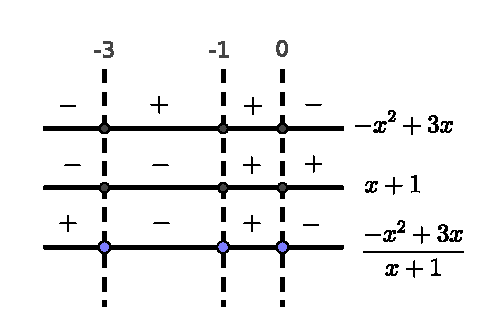
\includegraphics[width=8cm]{../Topicos/Figuras/sinais.pdf}
 \end{figure}
 
 Logo pelo jogo de sinais da figura acima, e considerando que a equação não pode ser calculada em $x= -1$, pois este número real zera o denominador, obtemos 
 \[S= [-3, -1) \cup [0, +\infty)\]
 como conjunto solução desta inequação.
  
 \end{exem}


 \section{Equações com módulo}% (fazendo)}

   \vskip0.3cm
 \colorbox{azul}{
 \begin{minipage}{0.9\linewidth}
 \begin{center}
  As equações modulares são equações que apresentam expressões algébricas dentro de um módulo.
 \end{center}
 \end{minipage}}
 \vskip0.3cm

 Antes de começarmos a ver exemplos destas equações lembremos que para um número real $x$ qualquer:

 \[
\abs{x}= \begin{cases}
      -x, \ \ \text{se} \ \ x<0 \\
      x, \ \ \text{se} \ \ x \geq 0 \ .
     \end{cases}
\]

Além disso o módulo de um número real possui algumas propriedades listadas na \autoref{prop.modulo} que serão necessárias para a resolução de equações modulares.

Vejamos então alguns exemplos de equações modulares resolvidas.

\begin{exem} Equações com módulo:
 \begin{enumerate}
  \item $\abs{x}= 10$

  Pela definição de módulo temos:
  \[
  \begin{cases}
      -x= 10, \ \ \text{se} \ \ x<0 \\
      x= 10, \ \ \text{se } \ \ x \geq 0 \ .
     \end{cases}
     \Rightarrow
     \begin{cases}
      x= -10, \ \ \text{se} \ \ x<0 \\
      x= 10, \ \ \text{se } \ \ x \geq 0 \ .
     \end{cases}
  \]

 \item $\abs{2x-2}= 10$

  Pela definição de módulo temos:
  \[
  \begin{cases}
      -(2x-2)= 10, \ \ \text{se} \ \ (2x-2)<0 \\
      2x-2= 10, \ \ \text{se } \ \ (2x-2) \geq 0
     \end{cases}
     \Rightarrow
     \begin{cases}
      -2x + 2= 10, \ \ \text{se} \ \ x< 1 \\
      2x - 2= 10, \ \ \text{se } \ \ x \geq 1
     \end{cases}
     \]
     \[
     \Rightarrow
     \begin{cases}
      -2x= 8, \ \ \text{se} \ \ x< 1 \\
       2x= 12, \ \ \text{se } \ \ x \geq 1
     \end{cases}
     \Rightarrow
     \begin{cases}
      x= -4, \ \ \text{se} \ \ x< 1 \\
      x= 6, \ \ \text{se } \ \ x \geq 1 \ .
     \end{cases}
  \]

  \item $\abs{2x^2 - 72}= 26$

  Novamente aplicando a definição de módulo temos
    \[
    \begin{cases}
      -(2x^2-72)= 26, \ \ \text{se} \ \ (2x^2-72)<0 \\
      2x^2- 72= 26, \ \ \text{se } \ \ (2x^2-72) \geq 0
     \end{cases}
     \]

     Como $2x^2- 72= 0 \Leftrightarrow 2x^2= 72 \Leftrightarrow x^2= 36 \Leftrightarrow \abs{x}= 6$ e a equação do 2º grau $2x^2- 72= 0$ tem $a> 0$, fazendo o estudo de sinal desta equação obtemos os três seguintes casos:
     \[
     \begin{cases}
      2x^2- 72 \geq 0, \ \ \text{se} \ \ x \leq -6 \\
      2x^2- 72 < 0, \ \ \text{se} \ \ -6 < x < 6 \\
      2x^2- 72 \geq 0, \ \ \text{se} \ \ x \geq 6 \\
     \end{cases}
     \]
     Com isso temos que a equação inicial deve ser dividida nos seguintes casos:
     \[
     \Rightarrow
      \begin{cases}
       2x^2- 72= 26, \ \ \text{se } \ \ x \leq -6 \\
      -(2x^2-72)= 26, \ \ \text{se} \ \ -6 < x < 6\\
       2x^2- 72= 26, \ \ \text{se } \ \ x \geq 6 \\
     \end{cases}
     \]
     temos portanto duas equações para resolver, façamos elas separadamente:
     \[2x^2- 72= 26 \Leftrightarrow 2x^2= 98 \Leftrightarrow x^2= 49 \Leftrightarrow x= \pm 7\]
     note que $-7 < -6$ e $7 > 6$ logo $x=-7$ e $x=7$ são soluções desta equação, agora vejamos o outro caso,
     \[-(2x^2-72)= 26 \Leftrightarrow -2x^2 + 72= 26 \Leftrightarrow -2x^2= -46 \Leftrightarrow x^2= 23 \Leftrightarrow x= \pm \sqrt{23} \approx \pm 4,78\]
     note que $-6< -\sqrt{23} < \sqrt{23} < 6$, logo $x=-\sqrt{23}$ e $x=\sqrt{23}$ são soluções desta equação. Portanto o conjunto solução da nossa é equação modular é:
     \[S= \{-7, -\sqrt{23}, \sqrt{23}, 7\} \ .\]

     \item \colorbox{yellow}{Contra-exemplo:} $\abs{x-4}=-2$

     Pela definição de módulo temos:
     \[
    \begin{cases}
      -(x-4)= -2, \ \ \text{se} \ \ (x-4) < 0 \\
        x-4 = -2, \ \ \text{se } \ \ (x-4) \geq 0
     \end{cases}
     \Rightarrow
     \begin{cases}
      -x+4= -2, \ \ \text{se} \ \ x < 4 \\
       x-4= -2, \ \ \text{se } \ \ x \geq 4
     \end{cases}
     \]
     \[
     \begin{cases}
      -x= -2-4, \ \ \text{se} \ \ x < 4 \\
       x= -2+4, \ \ \text{se } \ \ x \geq 4
     \end{cases}
     \Rightarrow
     \begin{cases}
      x= 6, \ \ \text{se} \ \ x < 4 \\
      x= 2, \ \ \text{se } \ \ x \geq 4
     \end{cases}
     \]
 Observe que em nenhum dos dois casos o $x$ encontrado pertence ao intervalo onde a solução deveria estar, pois $6$ não é menor que $4$ e $2$ não é maior ou igual a $4$, além disso,
 \[x=6 \Rightarrow \abs{6-4}= \abs{2}= 2 \neq -2\]
 \[x=2 \Rightarrow \abs{2-4}= \abs{-2}= 2 \neq -2\]
 logo esta equação NÃO tem solução!

 Mas isso já era de se esperar, pois lembra que $\abs{x}\geq 0$ para qualquer $x \in \R$, por propriedade do módulo, logo $\abs{x-4} \geq 0$ como $-2< 0$ então não existe $x \in \R$ tal que $\abs{x-4}= -2$. Portanto, já sabíamos pela propriedade de módulo que esta equação não tinha solução.

\end{enumerate}
\end{exem}

 Vamos agora, sistematizar o que acabamos de ver nos exemplos acima de forma a facilitar a aplicação desta teoria na resolução de equações modulares gerais. Para tal consideremos uma equação modular na forma geral
 \[\abs{A}= B\]
 em que $A$ e $B$ são expressões algébricas. Pela definição de módulo temos que
 \[ \abs{A}= \begin{cases}
          -A, \ \text{se} \ \ A < 0 \\
           A, \ \text{se} \ \ A \geq 0
         \end{cases}
 \]
 logo as soluções da equação modular devem satisfazer
 \[A= B \ \ \ \text{ou} \ \ \ -A= B \ .\]
 Além disso, lembremos que por propriedade de módulo $\abs{A}\geq 0$, então para ser uma solução da equação a variável $x$ deve também satisfazer esta propriedade. Mas como vimos no contra-exemplo acima nem toda variável satifaz
 \[(A= B \ \ \ \text{ou} \ \ \ -A= B) \ \ \ \text{e} \ \ \ (\abs{A}\geq 0) \ . \]
 Note que, como nossa equação é $\abs{A}= B$, logo garantir $\abs{A}\geq 0$ é equivalente a garantir $B \geq 0$, donde obtemos que as equações com $B < 0$ não possuem solução.

 Resumindo temos que,

  \vskip0.3cm
 \colorbox{rosa}{
 \begin{minipage}{0.9\linewidth}
 \begin{center}
   uma variável $x$ é solução da equação modular $\abs{A}= B$ se ela satisfizer:
 \[(A= B \ \ \ \text{ou} \ \ \ -A= B) \ \ \ \text{e} \ \ \ (B \geq 0) \ . \]
 \end{center}
 \end{minipage}}
 \vskip0.3cm
 
 Vejamos mais alguns exemplos resolvidos de equações com módulo.
 
 \begin{exem}
    $\abs{x-2} + \abs{x+4}= 10$
   
   Antes de começarmos a pensar em como resolver esta equação modular observe que $B= 10 \geq 0$, então uma das condições necessárias para se obter uma solução para a equação já está satisfeita, agora basta analisar os casos $A= B$ e $-A= B$. 
   
   Para fazer esta segunda etapa da solução lembre-se que no exemplo \autoref{eqmodulo} após simplificarmos a expressão $\abs{x-2} + \abs{x+4}$, considerando os casos $A< 0$, $A= 0$ e $A> 0$ e obtemos:
   \[ \abs{x-2} + \abs{x+4} = \begin{cases}
      -2x-2, \ \ \text{se} \ \ x < -4 \\
      6, \ \ \text{se } \ \ -4 \leq x < 2 \\
      2x + 2, \ \ \text{se} \ \ x \geq 2 \ .
     \end{cases}
  \]
 Agora para resolver esta equação modular vamos usar esta simplificação da expressão. Assim note que temos três casos para analisar, façamos eles separadamente.
 
 \textbf{Caso 1:} $x < -4$
 
 Neste caso, $\abs{x-2} + \abs{x+4}= -2x-2$, com isso temos que nossa equação se torna:
 \[-2x-2= 10 \Rightarrow -2x= 12 \Rightarrow x= -6\]
 como $x= -6$ satisfaz a inequação $x< -4$, ele é uma solução.
 
 \textbf{Caso 2:} $-4 \leq x < 2$
 
 Neste caso, $\abs{x-2} + \abs{x+4}= 6$, com isso temos que nossa equação se torna:
 \[6= 10\]
 o que é impossível, donde concluímos que neste intervalo a equação não tem solução.
 
 \textbf{Caso 3:} $x \geq 2 $
 
 Neste caso, $\abs{x-2} + \abs{x+4}= 2x + 2$, com isso temos que nossa equação se torna:
 \[2x + 2= 10 \Rightarrow 2x= 8 \Rightarrow x= 4\]
 como $x= 4$ satisfaz a inequação $x \geq 2$, ele é uma solução da equação.
 
 Portanto obtemos $S=\{-6, 4\}$ como conjunto solução da equação modular 
\[\abs{x-2} + \abs{x+4}= 10 \ .\]

 \end{exem}

 
 \section{Inequações modulares}% (fazer)}
 
 \begin{exem}
  \begin{enumerate}
  
   \item $\abs{x} \leq 5$
   \[\abs{x} \leq 5 \Leftrightarrow -5 \leq x \leq 5\]
   logo, o conjunto solução desta inequação é:
   \[S= [-5, 5] \ . \]
   
   \item $\abs{x} \geq 5$
   \[\abs{x} \geq 5 \Leftrightarrow x \leq -5 \ \ \text{ ou } \ \ x \geq 5\]
   logo, o conjunto solução desta inequação é:
   \[S= (-\infty, -5] \cup [5, \infty) \ . \]

  \end{enumerate}

 \end{exem}

 
% \section{Equações com raízes (fazer)}
 
% \section{Inequações com raízes (fazer)}
 

 
